\documentclass[a4paper,12pt,projekat]{etf}

\usepackage[intlimits]{amsmath}
\usepackage{amsmath, amsfonts, amssymb}
\usepackage{graphicx}
\usepackage{longtable}
\usepackage{array}
\usepackage{enumitem}
\usepackage{hyperref}
\usepackage{float}

\usepackage[serbian]{babel}
\usepackage[T1]{fontenc}
\usepackage[utf8]{inputenc}

\title{Geo Serbia \\ Backend and Frontend System Documentation}
\author{Aleksa Malezić}
\indeks{24/3124}
\date{13.03.2026}
\mentor{prof.~dr Milan Bjelica}
\predmet{Personalizovane Aplikacije}

\begin{document}

\maketitle

\begin{abstract}

GeoSerbia je web aplikacija inspirisana GeoGuessr igrom,
fokusirana na geografske lokacije u Srbiji. Korisnik dobija
fotografiju lokacije i treba da pogodi njenu poziciju na mapi.

Sistem se sastoji iz backend servisa implementiranog pomoću
FastAPI okvira i frontend aplikacije razvijene u Vue 3
tehnologiji. Backend je odgovoran za gameplay logiku,
autentifikaciju korisnika, leaderboard sistem i adaptivni
algoritam težine igre, dok frontend omogućava interaktivni
korisnički interfejs za igranje igre.

\end{abstract}

\begin{keywords}

FastAPI, Vue.js, PostgreSQL, geografske igre, web aplikacije, adaptivna težina

\end{keywords}

\tableofcontents

\chapter{Pregled sistema}

GeoSerbia je web aplikacija za geografski kviz.

Tok igre:

\begin{enumerate}

\item igrač dobija fotografiju lokacije
\item igrač bira lokaciju na mapi
\item sistem računa udaljenost
\item dodeljuju se poeni
\item igra se do pet rundi po danu
\item rezultat se čuva u leaderboard-u

\end{enumerate}

Sistem je podeljen na dve komponente:

\begin{itemize}

\item Backend servis
\item Frontend aplikacija

\end{itemize}

\chapter{Arhitektura sistema}

\begin{figure}[H]
\centering
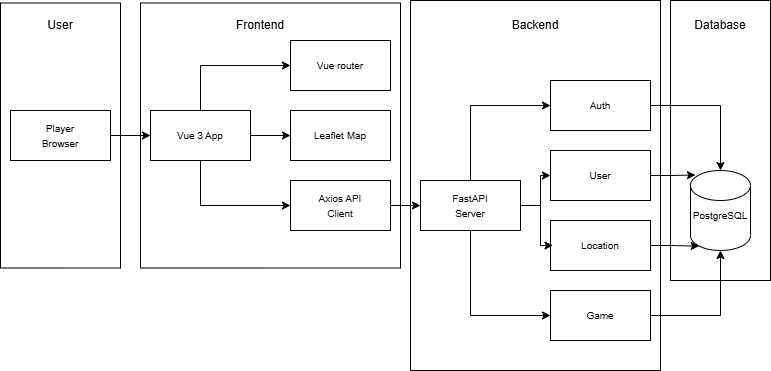
\includegraphics[width=0.8\textwidth]{architecture_diagram.png}
\caption{Opšta arhitektura sistema}
\end{figure}

Sistem koristi klijent-server arhitekturu.

\begin{itemize}

\item Frontend aplikacija komunicira sa backend API-jem
\item Backend pristupa PostgreSQL bazi
\item Autentifikacija koristi JWT tokene
\end{itemize}

\chapter{Backend sistem}

\section{Tehnologije}

Backend koristi sledeće tehnologije:

\begin{itemize}

\item FastAPI
\item Tortoise ORM
\item PostgreSQL
\item Aerich migracije
\item JWT autentifikacija
\item Pytest

\end{itemize}

\section{Struktura backend projekta}

\begin{verbatim}

backend/
  migrations/
  src/
    boot/
      main.py
    core/
      auth.py
      database.py
      security.py
      settings.py
    domains/
      users/
      locations/
      games/
      admin/
    scripts/
      seeders/
      tests/
  docker-compose.yml

\end{verbatim}

\section{Autentifikacija}

Backend koristi JWT autentifikaciju.

Tokeni se čuvaju u HTTP-only cookies.

Administratorske rute zahtevaju:

\begin{verbatim}
is_admin = True
\end{verbatim}

\chapter{Frontend sistem}

\section{Tehnologije}

Frontend koristi sledeće tehnologije:

\begin{itemize}

\item Vue 3
\item Vue Router
\item Axios
\item Leaflet
\item Vite

\end{itemize}

\section{Struktura projekta}

\begin{verbatim}

geo-serbia-frontend/
  src/
    api/
    components/
    composables/
    router/
    stores/
    views/
  public/
  package.json

\end{verbatim}

\chapter{Baza podataka}

\section{ER dijagram}

\begin{figure}[H]
\centering
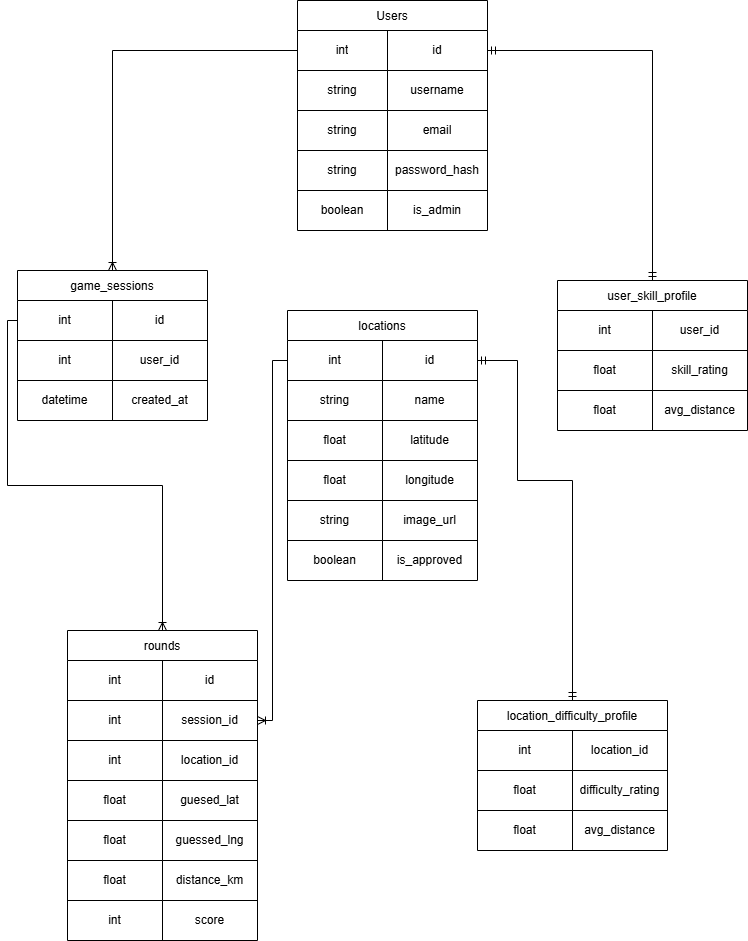
\includegraphics[width=0.9\textwidth]{database_er_diagram.png}
\caption{ER dijagram baze}
\end{figure}

Glavne tabele sistema:

\begin{itemize}

\item users
\item locations
\item game sessions
\item rounds
\item user skill profile
\item location difficulty profile

\end{itemize}

\chapter{Gameplay logika}

Svaka igra ima maksimalno pet rundi.

Poeni se računaju na osnovu udaljenosti između pogođene
i stvarne lokacije, kao i vremena trajanja runde.

\section{Haversine formula}

Za računanje udaljenosti koristi se Haversine formula:

\[
d = 2R \arcsin
\left(
\sqrt{
\sin^2\left(\frac{\phi_2-\phi_1}{2}\right)
+
\cos(\phi_1)\cos(\phi_2)
\sin^2\left(\frac{\lambda_2-\lambda_1}{2}\right)
}
\right)
\]

gde su:

\begin{itemize}

\item $\phi$ geografske širine
\item $\lambda$ geografske dužine
\item $R$ poluprečnik Zemlje

\end{itemize}

\chapter{Adaptivni sistem težine}

Sistem prilagođava težinu igre na osnovu
performansi korisnika i težine lokacija.

\section{Procena nivoa znanja korisnika}

Profil korisnika ažurira se nakon svake runde.
Sistem koristi poslednjih deset odigranih rundi.

Računaju se sledeće metrike:

\begin{itemize}

\item prosečan broj poena
\item prosečna udaljenost od tačne lokacije

\end{itemize}

Skill rating računa se formulom:

\[
skill = (avg\_points/5000)\cdot70 +
clamp(1 - avg\_distance/250,0,1)\cdot30
\]

Konačna vrednost skill rating-a nalazi se
u opsegu od 0 do 100.

\section{Težina lokacija}

Svaka lokacija ima procenjenu težinu
koja zavisi od:

\begin{itemize}

\item prosečne udaljenosti korisnika
\item prosečnog broja poena
\item broja pokušaja
\end{itemize}

Lokacije koje korisnici često pogađaju
sa velikom greškom smatraju se težim.

\section{Izbor lokacija}

U adaptivnom režimu igre:

\begin{enumerate}

\item očitava se skill rating korisnika
\item poredi se sa difficulty rating lokacija
\item bira se pet lokacija sa najmanjom razlikom

\end{enumerate}

Na ovaj način igra automatski prilagođava
težinu svakom korisniku.

% ----------------------------------------------------

\chapter{API komunikacija}

Frontend komunicira sa backend servisom
putem REST API-ja.

\section{Auth}

\begin{longtable}{|p{0.35\linewidth}|p{0.55\linewidth}|}
\hline
Endpoint & Opis \\
\hline
POST /api/v1/auth/login & login korisnika \\
POST /api/v1/auth/register & registracija \\
GET /api/v1/auth/me & podaci o korisniku \\
\hline
\end{longtable}

\section{Game}

\begin{longtable}{|p{0.35\linewidth}|p{0.55\linewidth}|}
\hline
Endpoint & Opis \\
\hline
POST /api/v1/game/start & pokretanje igre \\
POST /api/v1/game/play & slanje pokušaja \\
GET /api/v1/game/leaderboard/daily & dnevni leaderboard \\
GET /api/v1/game/leaderboard/monthly & mesečni leaderboard \\
\hline
\end{longtable}

% ----------------------------------------------------

\chapter{Request Flow}

\begin{figure}[H]
\centering
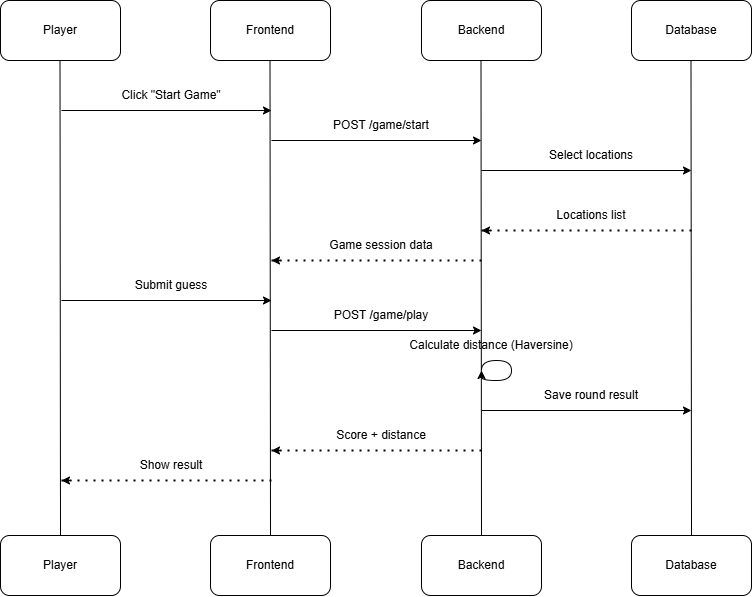
\includegraphics[width=0.9\textwidth]{flow_diagram.png}
\caption{Tok zahteva kroz sistem}
\end{figure}

Tipičan tok zahteva:

\begin{enumerate}

\item korisnik pokreće igru
\item frontend šalje zahtev backend-u
\item backend bira lokaciju
\item korisnik šalje guess
\item backend računa rezultat
\item rezultat se vraća frontend-u

\end{enumerate}

% ----------------------------------------------------

\chapter{Instalacija sistema}

\section{Backend}

\begin{verbatim}

python -m venv venv
venv\Scripts\activate
pip install -r requirements.txt
docker compose up -d
uvicorn src.boot.main:app --reload

\end{verbatim}

\section{Frontend}

\begin{verbatim}

npm install
npm run dev

\end{verbatim}

% ----------------------------------------------------

\chapter{Testiranje}

Backend testovi pokreću se komandom:

\begin{verbatim}

python -m pytest -q

\end{verbatim}

% ----------------------------------------------------

\chapter{Zaključak}

GeoSerbia predstavlja modularan full-stack sistem
za implementaciju geografske igre.

Sistem uključuje:

\begin{itemize}

\item autentifikaciju korisnika
\item gameplay mehanizam
\item leaderboard sistem
\item administrativne funkcionalnosti
\item adaptivni algoritam težine

\end{itemize}

Arhitektura sistema omogućava skalabilnost,
jednostavno održavanje i dalji razvoj.

\end{document}